% !TeX program = xelatex
\ifdefined\BookMaster\else
\documentclass[11pt,oneside]{article}
% !TeX program = xelatex
\usepackage[b5paper,left=22mm,right=22mm,top=20mm,bottom=22mm,footskip=11mm]{geometry}
\usepackage{fontspec}
\setmainfont{TeX Gyre Termes}
\setsansfont{TeX Gyre Heros}
\usepackage{amsmath,amssymb,mathtools,amsthm}
\renewcommand{\cdots}{\mathinner{\cdotp\cdotp\cdotp}}
\usepackage{graphicx,adjustbox,array,booktabs,longtable,multirow,enumitem,changepage,needspace}
\usepackage[table]{xcolor}
\usepackage{fancyhdr}
\raggedbottom
\interfootnotelinepenalty=10000
\newcommand{\BookFootnote}[2]{\begingroup\renewcommand{\thefootnote}{\fnsymbol{footnote}}\footnote[#1]{#2}\endgroup}
\newcommand{\BookFootnoteMark}[1]{\begingroup\renewcommand{\thefootnote}{\fnsymbol{footnote}}\footnotemark[#1]\endgroup}
\newcommand{\BookFootnoteText}[2]{\begingroup\renewcommand{\thefootnote}{\fnsymbol{footnote}}\footnotetext[#1]{#2}\endgroup}
\newenvironment{BookFloat}[1]{\par\addvspace{.6\baselineskip}\noindent\def\BookFloatID{#1}\begin{minipage}{\linewidth}\phantomsection\label{bookfloat:#1:start}}{\phantomsection\label{bookfloat:\BookFloatID:end}\end{minipage}\par\addvspace{.6\baselineskip}}

\usepackage[unicode,hidelinks]{hyperref}
\pagestyle{fancy}
\fancyhf{}
\newcommand{\BookFooter}{}
\fancyfoot[L]{\parbox[b]{\dimexpr\textwidth-15mm}{\footnotesize\BookFooter}}
\fancyfoot[R]{\footnotesize\thepage}
\renewcommand{\headrulewidth}{0pt}
\renewcommand{\footrulewidth}{0pt}
\setlength{\parindent}{0pt}
\setlength{\parskip}{0.2em}
\setlength{\emergencystretch}{3em}
\setlist{nosep,leftmargin=1.7em,labelsep=.65em}
\newif\ifBookNarrative
\BookNarrativetrue
\newenvironment{BookBody}{\setlength{\parindent}{0pt}}{}
\newcommand{\BookStatement}[1]{\par\addvspace{.6\baselineskip}\noindent #1\enspace\ignorespaces}
\newcommand{\BookLabel}[1]{\par\addvspace{.6\baselineskip}\needspace{3\baselineskip}\noindent\textbf{#1}\quad\ignorespaces}
\newcommand{\BookHeading}[1]{\par\addvspace{\baselineskip}\needspace{4\baselineskip}\noindent{\large\bfseries #1}\par\medskip}
\newcommand{\BookSubheading}[1]{\par\addvspace{.7\baselineskip}\needspace{3\baselineskip}\noindent{\bfseries #1}\par\smallskip}
\newcommand{\BookTextHeading}[1]{\par\addvspace{.7\baselineskip}\needspace{3\baselineskip}\noindent #1\par\smallskip}
\newcommand{\BookSectionTitle}[2]{\par\addvspace{1.2\baselineskip}\needspace{5\baselineskip}\noindent\colorbox{gray!25}{\sffamily\bfseries\small SECTION #1}\quad{\large\bfseries #2}\par\medskip}
\newcommand{\BookExerciseTitle}[1]{\par\addvspace{\baselineskip}\needspace{4\baselineskip}\noindent{\color{gray}\rule{1.5mm}{1.5mm}}\enspace{\large\bfseries Exercises #1}\par\medskip}
\newcommand{\BookBullet}[1]{\begin{list}{\textbullet}{\setlength{\leftmargin}{1.7em}\setlength{\labelwidth}{1em}\setlength{\labelsep}{.7em}\setlength{\topsep}{0pt}\setlength{\parsep}{0pt}\setlength{\itemsep}{0pt}}\item #1\end{list}}
\newcommand{\BookExercise}[2]{\begin{list}{\textbf{#1}}{\setlength{\leftmargin}{2.2em}\setlength{\labelwidth}{1.5em}\setlength{\labelsep}{.7em}\setlength{\topsep}{.15em}\setlength{\parsep}{0pt}\setlength{\itemsep}{0pt}}\item #2\end{list}}
\newcommand{\BookEnd}[1]{\unskip\nobreak\hfill\ensuremath{#1}}
\newcommand{\BookSource}[2]{\phantomsection\label{sourcepage:#1}} % Source-page anchors, retained through reflow.
\usepackage{multicol}
\usepackage{tikz}
\newcommand{\BookPartEntry}[2]{\par\noindent\makebox[17mm][l]{\bfseries Section #1}#2\par}
\newcommand{\BookPartTitle}[3]{\par\bigskip\noindent\begin{tikzpicture}\node[anchor=north west,inner sep=0pt,outer sep=0pt] (bookpart) at (0,0) {\begin{minipage}{\dimexpr\linewidth-.5pt}\hspace*{26mm}\begin{minipage}[t]{\dimexpr\linewidth-26mm}\begin{adjustbox}{max width=\linewidth}{\fontsize{20}{24}\selectfont\bfseries #2}\end{adjustbox}\par\vspace{6mm}\hrule\vspace{6mm}{\sffamily\footnotesize\setlength{\parskip}{.3em}#3}\vspace{3mm}\end{minipage}\end{minipage}};\path[shade,top color=gray!60,bottom color=white] (0,0) rectangle ([xshift=24mm]bookpart.south west);\node[anchor=north,font=\sffamily\bfseries\small] at (12mm,-2mm) {PART};\node[anchor=north,font=\sffamily\bfseries\Huge] at (12mm,-7mm) {#1};\end{tikzpicture}\par\bigskip}
\newsavebox{\BookMathBox}
\makeatletter
\newcommand{\BookInline}[1]{\leavevmode\hskip0pt\relax\begingroup\in@{\begin}{#1}\ifin@\sbox{\BookMathBox}{\(#1\)}\ifdim\wd\BookMathBox>\dimexpr\linewidth-1em\relax\resizebox{\dimexpr\linewidth-1em\relax}{!}{\usebox{\BookMathBox}}\else\(#1\)\fi\else\in@{\left}{#1}\ifin@\sbox{\BookMathBox}{\(#1\)}\ifdim\wd\BookMathBox>\dimexpr\linewidth-1em\relax\resizebox{\dimexpr\linewidth-1em\relax}{!}{\usebox{\BookMathBox}}\else\(#1\)\fi\else\(#1\)\fi\fi\endgroup\hskip0pt\relax}
\makeatother
\DeclareMathOperator{\Aut}{Aut}
\DeclareMathOperator{\End}{End}
\DeclareMathOperator{\Hom}{Hom}
\DeclareMathOperator{\GF}{GF}
\DeclareMathOperator{\irr}{irr}
\DeclareMathOperator{\lt}{lt}
\DeclareMathOperator{\lp}{lp}
\providecommand{\textcircled}[1]{\textnormal{(#1)}}

\begin{document}
\fi
\renewcommand{\BookFooter}{Section 4 Nonabelian Examples}
\pdfbookmark[0]{Section 4 Nonabelian Examples}{04_nonabelian_examples}
\ifdefined\BookMaster\else\setcounter{page}{39}\fi
% Source PDF page 56; original printed page 39
\BookSource{56}{39}
\BookNarrativetrue

\begin{BookBody}

\BookSectionTitle{4}{Nonabelian Examples}

\BookTextHeading{\textbf{Notation and Terminology}  }

\noindent It is time to explain some conventional notation and terminology used in group theory. Algebraists as a rule do not use a special symbol \BookInline{\ast } to denote a binary operation different from the usual addition and multiplication. They stick with the conventional additive or multiplicative notation and even call the operation\textit{ addition} or\textit{ multiplication,} depending 
% Source PDF page 57; original printed page 40
\BookSource{57}{40}
on the symbol used. The symbol for addition is, of course\BookInline{,\allowbreak +,\allowbreak } and usually multiplication is denoted by juxtaposition without a dot, if no confusion results. Thus in place of the notation \BookInline{a\ast b,\allowbreak } we shall be using either \BookInline{a+ b} to be read “the\textit{ sum} of \BookInline{a} and \BookInline{b,\allowbreak }” or \BookInline{ab} to be read “the\textit{ product} of \BookInline{a} and \BookInline{b.}” There is a sort of unwritten agreement that the symbol \BookInline{+ } should be used only to designate commutative operations. Algebraists feel very uncomfortable when they see \BookInline{a+ b\neq b+ a.} For this reason, when developing our theory in a general situation where the operation may or may not be commutative, we shall always use multiplicative notation.

\end{BookBody}

\BookNarrativetrue

\begin{BookBody}

Algebraists frequently use the symbol 0 to denote an additive identity element and the symbol 1 to denote a multiplicative identity element, even though they may not be actually denoting the integers 0 and 1. Of course, if they are also talking about numbers at the same time, so that confusion would result, symbols such as \BookInline{e} or \BookInline{u} are used as identity elements. Thus a table for a group of three elements might be one like Table 4.1 or, since such a group is commutative, the table might look like Table 4.2. In general situations we shall continue to use \BookInline{e} to denote the identity element of a group.

\begin{BookFloat}{04_nonabelian_examples-p57-2}
\begin{center}\small\textbf{4.1 Table}\end{center}
\begin{center}\begin{adjustbox}{max width=\linewidth}
\renewcommand{\arraystretch}{1.2}\setlength{\tabcolsep}{5pt}
\begin{tabular}{c|c|c|c}
 & 1 & \BookInline{a} & \BookInline{b}\\\hline
1 & 1 & \BookInline{a} & \BookInline{b}\\\hline
\BookInline{a} & \BookInline{a} & \BookInline{b} & 1\\\hline
\BookInline{b} & \BookInline{b} & 1 & \BookInline{a}\\
\end{tabular}
\end{adjustbox}\end{center}
\end{BookFloat}

It is customary to denote the inverse of an element \BookInline{a} in a group by \BookInline{a^{- 1}} in multiplicative notation and by \BookInline{- a} in additive notation. From now on, we shall use these notations in place of the symbol \BookInline{a^{\prime }.}

Let \BookInline{n} be a positive integer. If \BookInline{a} is an element of a group \BookInline{G,\allowbreak } written multiplicatively, we denote the product \BookInline{aaa...a} for \BookInline{n} factors \BookInline{a} by \BookInline{a^{n}.} We let \BookInline{a^{0}} be the identity element \BookInline{e,\allowbreak } and denote the product \BookInline{a^{- 1}a^{- 1}a^{- 1}...a^{- 1}} for \BookInline{n} factors by \BookInline{a^{- n}.} It is easy to see that our usual law of exponents\BookInline{,\allowbreak a^{m}a^{n}= a^{m+ n}} for \BookInline{m,\allowbreak n\in \mathbb{Z},\allowbreak } holds. For \BookInline{m,\allowbreak n\in \mathbb{Z}^{+ },\allowbreak } it is clear. We illustrate another type of case by an example:

\begin{BookFloat}{04_nonabelian_examples-p57-5}
\begin{center}\small\textbf{4.2 Table}\end{center}
\begin{center}\begin{adjustbox}{max width=\linewidth}
\renewcommand{\arraystretch}{1.2}\setlength{\tabcolsep}{5pt}
\begin{tabular}{c|c|c|c}
\BookInline{+ } & 0 & \BookInline{a} & \BookInline{b}\\\hline
0 & 0 & \BookInline{a} & \BookInline{b}\\\hline
\BookInline{a} & \BookInline{a} & \BookInline{b} & 0\\\hline
\BookInline{b} & \BookInline{b} & 0 & \BookInline{a}\\
\end{tabular}
\end{adjustbox}\end{center}
\end{BookFloat}

\begin{center}\begin{adjustbox}{max width=\linewidth}\BookInline{\displaystyle \begin{aligned}a^{- 2}a^{5}&= a^{- 1}a^{- 1}aaaaa= a^{- 1}(a^{- 1}a)aaaa= a^{- 1}eaaaa= a^{- 1}(ea)aaa \\ &= a^{- 1}aaaa= (a^{- 1}a)aaa= eaaa= (ea)aa= aaa= a^{3}.\end{aligned}}\end{adjustbox}\end{center}

\noindent In additive notation, we denote \BookInline{a+ a+ a+ \cdots + a} for \BookInline{n} summands by \BookInline{na,\allowbreak } denote \BookInline{(- a)+ (- a)+ (- a)+ \cdots + (- a)} for \BookInline{n} summands by \BookInline{- na,\allowbreak } and let \BookInline{0a} be the identity element. Be careful: In the notation \BookInline{na,\allowbreak } the number \BookInline{n} is in \BookInline{\mathbb{Z},\allowbreak } not in \BookInline{G.} One reason we prefer to present group theory using multiplicative notation, even if \BookInline{G} is abelian, is the confusion caused by regarding \BookInline{n} as being in \BookInline{G} in this notation \BookInline{na.} No one ever misinterprets the \BookInline{n} when it appears in an exponent.

The following table summarizes basic notations and facts using both additive and multiplicative notation. We assume that \BookInline{a} is an element of a group\BookInline{,\allowbreak n,\allowbreak m} are integers, and \BookInline{k} is a positive integer.

\begin{BookFloat}{04_nonabelian_examples-p57-9}
\begin{center}\begin{adjustbox}{max width=\linewidth}
\begin{tabular}{|c|c|c|}\hline
$\ast$ Notation & $+$ Notation & $\cdot$ Notation\\\hline
May or may not be abelian & Abelian & May or may not be abelian\\\hline
$e$ & $0$ & $1$\\\hline
$a'$ & $-a$ & $a^{-1}$\\\hline
$a\ast b$ & $a+b$ & $ab$\\\hline
$\underbrace{a\ast a\ast\cdots\ast a}_{k}$ & $ka$ & $a^k$\\\hline
$\underbrace{(a'\ast a'\ast\cdots\ast a')}_{k}$ & $-ka$ & $a^{-k}$\\\hline
& $0a=0$ & $a^0=1$\\\hline
& $(n+m)a=na+ma$ & $a^{n+m}=a^n a^m$\\\hline
& $n(ma)=(nm)a$ & $(a^n)^m=a^{nm}$\\\hline
\end{tabular}\end{adjustbox}\end{center}
\end{BookFloat}

Typically when stating a theorem we will use multiplicative notation, but the theorem also applies when using additive notation by using the above table to translate.

\end{BookBody}

% Source PDF page 58; original printed page 41
\BookSource{58}{41}
\BookNarrativetrue

\begin{BookBody}

We often refer to the number of elements in a group, so we have a term for this number.

\BookLabel{4.3 Definition} If \BookInline{G} is a group, then the\textbf{ order} of \BookInline{G} is the number of elements or cardinality of \BookInline{G.} The order of \BookInline{G} is denoted \BookInline{|G|.}\BookEnd{\blacksquare}

\BookTextHeading{\textbf{Permutations}}

\noindent We have seen examples of groups of numbers, like the groups \BookInline{\mathbb{Z},\allowbreak \mathbb{Q},\allowbreak } and \BookInline{\mathbb{R}} under addition. We have also introduced groups of matrices, like the group\textit{ GL}\BookInline{(2,\allowbreak \mathbb{R}).} Each element \BookInline{A} of\textit{ GL}\BookInline{(2,\allowbreak \mathbb{R})} yields a transformation of the plane \BookInline{\mathbb{R}^{2}} into itself; namely, if we regard \textbf{x} as a 2-component column vector, then \BookInline{A}\textbf{x} is also a 2-component column vector. The group\textit{ GL}\BookInline{(2,\allowbreak \mathbb{R})} is typical of many of the most useful groups in that its elements\textit{ act} \textit{on things} to transform them. Often, an action produced by a group element can be regarded as a\textit{ function}, and the binary operation of the group can be regarded as\textit{ function} \textit{composition}. In this section, we construct some finite groups whose elements, called \textit{permutations}, act on finite sets. These groups will provide us with examples of finite nonabelian groups.

You may be familiar with the notion of a permutation of a set as a rearrangement of the elements of the set. Thus for the set \BookInline{\{1,\allowbreak 2,\allowbreak 3,\allowbreak 4,\allowbreak 5\},\allowbreak } a rearrangement of the elements could be given schematically as in Fig. 4.4, resulting in the new arrangement \BookInline{\{4,\allowbreak 2,\allowbreak 5,\allowbreak } \BookInline{3,\allowbreak 1\}.} Let us think of this schematic diagram in Fig. 4.4 as a function mapping each element listed in the left column into a single (not necessarily different) element from the same set listed at the right. Thus 1 is carried into 4, 2 is mapped into 2, and so on. Furthermore, to be a permutation of the set, this mapping must be such that each element appears in the right column once and only once. For example, the diagram in Fig. 4.5 does\textit{ not} give a permutation, for 3 appears twice while 1 does not appear at all in the right column. We now define a permutation to be such a mapping.

\begin{center}\begin{adjustbox}{max width=\linewidth}\BookInline{\displaystyle \begin{aligned}&1\to 41\to 3 \\ &2\to 22\to 2 \\ &3\to 53\to 4 \\ &4\to 34\to 5 \\ &5\to 15\to 3 \\ &4.4\;\text{Figure}\;4.5\;\text{Figure}\;\end{aligned}}\end{adjustbox}\end{center}

\BookLabel{4.6 Definition} A\textbf{ permutation of a set} \BookInline{A} is a function \BookInline{\phi:A\to A} that is both one-to-one and onto. \BookEnd{\blacksquare}

\BookTextHeading{\textbf{Permutation Groups}  }

\noindent We now show that function composition \BookInline{\circ } is a binary operation on the collection of all permutations of a set \BookInline{A.} We call this operation\textit{ permutation multiplication}. Let \BookInline{A} be a set, and let \BookInline{\sigma } and \BookInline{\tau } be permutations of \BookInline{A} so that \BookInline{\sigma } and \BookInline{\tau } are both one-to-one functions mapping \BookInline{A} onto \BookInline{A.} The composite function \BookInline{\sigma \circ \tau } defined schematically by

\begin{center}\begin{adjustbox}{max width=\linewidth}\BookInline{\displaystyle A\to ^{\tau }A\to ^{\sigma }A,\allowbreak }\end{adjustbox}\end{center}

\noindent gives a mapping of \BookInline{A} into \BookInline{A.} Rather than keep the symbol \BookInline{\circ } for permutation multiplication, we will denote \BookInline{\sigma \circ \tau } by the juxtaposition \BookInline{\sigma \tau.} Now \BookInline{\sigma \tau } will be a permutation if it is one-to-one and onto \BookInline{A.} \textit{Remember that the action of} \BookInline{\sigma \tau } \textit{on} \BookInline{A} \textit{must be read in} \textit{right-to-left order}\BookInline{:\text{fi}rst} \textit{apply} \BookInline{\tau } \textit{and then} \BookInline{\sigma.} Let us show that \BookInline{\sigma \tau } is one-to-one. If

\begin{center}\begin{adjustbox}{max width=\linewidth}\BookInline{\displaystyle (\sigma \tau )(a_{1})= (\sigma \tau )(a_{2}),\allowbreak }\end{adjustbox}\end{center}

\end{BookBody}

% Source PDF page 59; original printed page 42
\BookSource{59}{42}
\BookNarrativetrue

\begin{BookBody}

\noindent then

\begin{center}\begin{adjustbox}{max width=\linewidth}\BookInline{\displaystyle \sigma (\tau (a_{1}))= \sigma (\tau (a_{2})),\allowbreak }\end{adjustbox}\end{center}

\noindent and since \BookInline{\sigma } is given to be one-to-one, we know that \BookInline{\tau (a_{1})= \tau (a_{2}).} But then, since \BookInline{\tau } is one-to-one, this gives \BookInline{a_{1}= a_{2}.} Hence \BookInline{\sigma \tau } is one-to-one. To show that \BookInline{\sigma \tau } is onto \BookInline{A,\allowbreak } let \BookInline{a\in A.} Since \BookInline{\sigma } is onto \BookInline{A,\allowbreak } there exists \BookInline{a^{\prime }\in A} such that \BookInline{\sigma (a^{\prime })= a.} Since \BookInline{\tau } is onto \BookInline{A,\allowbreak } there exists \BookInline{a^{\prime \prime }\in A} such that \BookInline{\tau (a^{\prime \prime })= a^{\prime }.} Thus

\begin{center}\begin{adjustbox}{max width=\linewidth}\BookInline{\displaystyle a= \sigma (a^{\prime })= \sigma (\tau (a^{\prime \prime }))= (\sigma \tau )(a^{\prime \prime }),\allowbreak }\end{adjustbox}\end{center}

\noindent so \BookInline{\sigma \tau } is onto \BookInline{A.}

\BookLabel{4.7 Example} Suppose that

\begin{center}\begin{adjustbox}{max width=\linewidth}\BookInline{\displaystyle A= \{1,\allowbreak 2,\allowbreak 3,\allowbreak 4,\allowbreak 5\}}\end{adjustbox}\end{center}

\noindent and that \BookInline{\sigma } is the permutation given by Fig. 4.4. We write \BookInline{\sigma } in a more standard notation, changing the columns to rows in parentheses and omitting the arrows, as

\begin{center}\begin{adjustbox}{max width=\linewidth}\BookInline{\displaystyle \sigma = \begin{pmatrix} 1 & 2 & 3 & 4 & 5 \\ 4 & 2 & 5 & 3 & 1 \end{pmatrix},\allowbreak }\end{adjustbox}\end{center}

\noindent so that \BookInline{\sigma (1)= 4,\allowbreak \sigma (2)= 2,\allowbreak } and so on. Let

\begin{center}\begin{adjustbox}{max width=\linewidth}\BookInline{\displaystyle \tau = \begin{pmatrix} 1 & 2 & 3 & 4 & 5 \\ 3 & 5 & 4 & 2 & 1 \end{pmatrix}.}\end{adjustbox}\end{center}

\noindent Then

\begin{center}\begin{adjustbox}{max width=\linewidth}\BookInline{\displaystyle \sigma \tau = \begin{pmatrix} 1 & 2 & 3 & 4 & 5 \\ 4 & 2 & 5 & 3 & 1 \end{pmatrix} \begin{pmatrix} 1 & 2 & 3 & 4 & 5 \\ 3 & 5 & 4 & 2 & 1 \end{pmatrix} = \begin{pmatrix} 1 & 2 & 3 & 4 & 5 \\ 5 & 1 & 3 & 2 & 4 \end{pmatrix}.}\end{adjustbox}\end{center}

\noindent For example, multiplying in right-to-left order,

\begin{center}\begin{adjustbox}{max width=\linewidth}\BookInline{\displaystyle (\sigma \tau )(1)= \sigma (\tau (1))= \sigma (3)= 5.}\end{adjustbox}\end{center} \BookEnd{\blacktriangle}

\BookTextHeading{\ensuremath{\blacksquare} \textbf{HISTORICAL NOTE}  }

\noindent One of the earliest recorded studies of permutations occurs in the\textit{ Sefer Yetsirah,} or \textit{Book of Creation,} written by an unknown Jewish author sometime before the eighth century. The author was interested in counting the various ways in which the letters of the Hebrew alphabet can be arranged. The question was in some sense a mystical one. It was believed that the letters had magical powers; therefore, suitable arrangements could subjugate the forces of nature. The actual text of the \textit{Sefer Yetsirah} is very sparse: “Two letters build two words, three build six words, four build 24 words, five build 120, six build 720, seven build 5040.” Interestingly enough, the idea of counting the arrangements of the letters of the alphabet also occurred in Islamic mathematics in the eighth and ninth centuries. By the thirteenth century, in both the Islamic and Hebrew cultures, the abstract idea of a permutation had taken root so that both Abul-’ Abbas ibn al-Banna (1256–1321), a mathematician from Marrakech in what is now Morocco, and Levi ben Gerson, a French rabbi, philosopher, and mathematician, were able to give rigorous proofs that the number of permutations of any set of \BookInline{n} elements is \BookInline{n}!, as well as prove various results about counting combinations.

Levi and his predecessors, however, were concerned with permutations as simply arrangements of a given finite set. It was the search for solutions of polynomial equations that led Lagrange and others in the late eighteenth century to think of permutations as functions from a finite set to itself, the set being that of the roots of a given equation. And it was Augustin-Louis Cauchy (1789–1857) who developed in detail the basic theorems of permutation theory and who introduced the standard notation used in this text.

\end{BookBody}

% Source PDF page 60; original printed page 43
\BookSource{60}{43}
\BookNarrativetrue

\begin{BookBody}

We now show that the collection of all permutations of a nonempty set A forms a group under this permutation multiplication.

\BookLabel{4.8 Theorem} Let \BookInline{A} be a nonempty set, and let \BookInline{S_{A}} be the collection of all permutations of \BookInline{A.} Then \BookInline{S_{A}} is a group under permutation multiplication.

\BookLabel{\textit{Proof}} We have shown that composition of two permutations of \BookInline{A} yields a permutation of \BookInline{A,\allowbreak } so \BookInline{S_{A}} is closed under permutation multiplication.

Now permutation multiplication is defined as function composition, and in Section 1, we showed that\textit{ function composition is associative}. Hence \BookInline{\mathcal{G}_{1}} is satisfied.

The permutation \BookInline{\iota } such that \BookInline{\iota (a)= a,\allowbreak } for all \BookInline{a\in A} acts as identity. Therefore \BookInline{\mathcal{G}_{2}} is satisfied.

For a permutation \BookInline{\sigma,\allowbreak } the inverse function\BookInline{,\allowbreak \sigma ^{- 1},\allowbreak } is the permutation that reverses the direction of the mapping \BookInline{\sigma,\allowbreak } that is\BookInline{,\allowbreak \sigma ^{- 1}(a)} is the element \BookInline{a^{\prime }} of \BookInline{A} such that \BookInline{a= \sigma (a^{\prime }).} The existence of exactly one such element \BookInline{a^{\prime }} is a consequence of the fact that, as a function\BookInline{,\allowbreak \sigma } is both one-to-one and onto. For each \BookInline{a\in A} we have

\begin{center}\begin{adjustbox}{max width=\linewidth}\BookInline{\displaystyle \iota (a)= a= \sigma (a^{\prime })= \sigma (\sigma ^{- 1}(a))= (\sigma \sigma ^{- 1})(a)}\end{adjustbox}\end{center}

\noindent and also

\begin{center}\begin{adjustbox}{max width=\linewidth}\BookInline{\displaystyle \iota (a^{\prime })= a^{\prime }= \sigma ^{- 1}(a)= \sigma ^{- 1}(\sigma (a^{\prime }))= (\sigma ^{- 1}\sigma )(a^{\prime }),\allowbreak }\end{adjustbox}\end{center}

\noindent so that \BookInline{\sigma ^{- 1}\sigma } and \BookInline{\sigma \sigma ^{- 1}} are both the permutation \BookInline{\iota.} Thus \BookInline{\mathcal{G}_{3}} is satisfied. \BookEnd{\blacklozenge}

\noindent \textbf{Warning:} Some texts compute a product \BookInline{\sigma \mu } of permutations in left-to-right order, so that \BookInline{(\sigma \mu )(a)= \mu (\sigma (a)).} Thus the permutation they get for \BookInline{\sigma \mu } is the one we would get by computing \BookInline{\mu \sigma.} Exercise 34 asks us to check in two ways that we still get a group. If you refer to another text on this material, be sure to check its order for permutation multiplication.

There was nothing in our definition of a permutation to require that the set \BookInline{A} be finite. However, most of our examples of permutation groups will be concerned with permutations of finite sets. Note that the\textit{ structure} of the group \BookInline{S_{A}} is concerned only with the number of elements in the set \BookInline{A,\allowbreak } and not what the elements in \BookInline{A} are. If sets \BookInline{A} and \BookInline{B} have the same cardinality, then \BookInline{S_{A}\simeq S_{B}.} To define an isomorphism \BookInline{\phi:S_{A}\to S_{B},\allowbreak } we let \BookInline{f:A\to B} be a one-to-one function mapping \BookInline{A} onto \BookInline{B,\allowbreak } which establishes that \BookInline{A} and \BookInline{B} have the same cardinality. For \BookInline{\sigma \in S_{A},\allowbreak } we let \BookInline{\phi (\sigma )} be the permutation \BookInline{\overline{\sigma }\in S_{B}} such that \BookInline{\overline{\sigma }(f(a))= f(\sigma (a))} for all \BookInline{a\in A.} To illustrate this for \BookInline{A= \{1,\allowbreak 2,\allowbreak 3\}} and \BookInline{B= \{}\#, \$, \%\BookInline{\}} and the function \BookInline{f:A\to B} defined as

\begin{center}\begin{adjustbox}{max width=\linewidth}\BookInline{\displaystyle f(1)= \#,\allowbreak f(2)= \$,\allowbreak f(3)= \%,\allowbreak }\end{adjustbox}\end{center}

\noindent \BookInline{\phi } maps

\begin{center}\begin{adjustbox}{max width=\linewidth}\BookInline{\displaystyle \begin{pmatrix}1 & 2 & 3 \\3 & 2 & 1\end{pmatrix}\;\mathrm{into}\;\begin{pmatrix}\# & \S & \% \\\% & \S & \#\end{pmatrix}.}\end{adjustbox}\end{center}

\noindent We simply rename the elements of \BookInline{A} in our two-row notation by elements in \BookInline{B} using the renaming function \BookInline{f,\allowbreak } thus renaming elements of \BookInline{S_{A}} to be those of \BookInline{S_{B}.} We can take \BookInline{\{1,\allowbreak 2,\allowbreak 3,\allowbreak \cdots,\allowbreak } n\BookInline{\}} to be a prototype for a finite set \BookInline{A} of \BookInline{n} elements.

\BookLabel{4.9 Definition} Let \BookInline{A} be the finite set \BookInline{\{1,\allowbreak 2,\allowbreak \cdots,\allowbreak n\}.} The group of all permutations of \BookInline{A} is the\textbf{ symmetric} \textbf{group on} \BookInline{n} \textbf{letters}, and is denoted by \BookInline{S_{n}.}\BookEnd{\blacksquare}

\noindent Note that \BookInline{S_{n}} has \BookInline{n}! elements, where

\begin{center}\begin{adjustbox}{max width=\linewidth}\BookInline{\displaystyle n!= n(n- 1)(n- 2)\cdots (3)(2)(1).}\end{adjustbox}\end{center}

\end{BookBody}

% Source PDF page 61; original printed page 44
\BookSource{61}{44}
\BookNarrativetrue

\begin{BookBody}

\begin{center}\begin{adjustbox}{max width=\linewidth}\BookInline{\displaystyle \begin{aligned}\operatorname{Let} \sigma = \binom{1\ 2\ 3}{2\ 1\ 3}\  and  \tau = \binom{1\ 2\ 3}{1\ 3\ 2}.  Then  \\\sigma \tau(1) = \sigma(1) = 2.\end{aligned}}\end{adjustbox}\end{center}

\noindent and

\begin{center}\begin{adjustbox}{max width=\linewidth}\BookInline{\displaystyle \tau \sigma (1)= 3}\end{adjustbox}\end{center}

\noindent which says that \BookInline{\sigma \tau \neq \tau \sigma.} Therefore \BookInline{S_{3}} is not abelian. We have seen that any group with at most four elements is abelian. Furthermore we will see later that up to isomorphism, the abelian group \BookInline{\mathbb{Z}_{5}} is the only group of order 5. Thus \BookInline{S_{3}} is the smallest group which is not abelian.

Suppose that \BookInline{\sigma = \begin{pmatrix} 1\ 2\ 3\ 4\ 5\ 6 \\ 3\ 2\ 6\ 1\ 4\ 5 \end{pmatrix}}. We find the inverse \BookInline{\sigma ^{- 1}.} We saw in the proof of Theorem 4.8 that the inverse function of a permutation is the group inverse. So it is easy to find inverses for permutations, we simply turn the tables! That is, we switch the top and bottom rows and sort the columns so the top row is in order:

\BookLabel{4.10 Example} 

\begin{center}\begin{adjustbox}{max width=\linewidth}\BookInline{\displaystyle \sigma^{-1} = \begin{pmatrix} 1\ 2\ 3\ 4\ 5\ 6 \\ 4\ 2\ 1\ 5\ 6\ 3 \end{pmatrix}.}\end{adjustbox}\end{center} \BookEnd{\blacktriangle}

\BookTextHeading{\textbf{Disjoint Cycles}  }

\noindent There is a more efficient way of specifying the action of a permutation. In the two-row notation that we have been using, we list each number 1 through \BookInline{n} twice, once in the top row and once in the bottom row. Disjoint cycle notation allows us to write the permutation using each number only once. We illustrate with an example. Let \BookInline{\sigma = } \BookInline{\begin{pmatrix}1 2 3 4 5 6 \\3 4 6 2 5 1\end{pmatrix}}. To write in disjoint cycle notation we start by writing

(1

\noindent We see that \BookInline{\sigma (1)= 3,\allowbreak } so we place 3 just to the right of 1:

\begin{center}\begin{adjustbox}{max width=\linewidth}\BookInline{\displaystyle (1,\allowbreak 3}\end{adjustbox}\end{center}

\noindent Now we see that \BookInline{\sigma } maps 3 to 6, so we write:

\begin{center}\begin{adjustbox}{max width=\linewidth}\BookInline{\displaystyle (1,\allowbreak 3,\allowbreak 6}\end{adjustbox}\end{center}

\noindent Our permutation maps 6 to 1, but there is no reason to write 1 again, so we just place a parenthesis after the 6 to indicate that 6 maps back to the first element listed:

\begin{center}\begin{adjustbox}{max width=\linewidth}\BookInline{\displaystyle (1,\allowbreak 3,\allowbreak 6)}\end{adjustbox}\end{center}

This is called a\textbf{ cycle} because when we apply \BookInline{\sigma } repeatedly, we cycle through the numbers 1, 3, and 6. A cycle containing exactly \BookInline{k} numbers is called a \BookInline{k-}\textbf{cycle}. So the cycle (1, 3, 6) is a 3-cycle. This is not the end of the story for \BookInline{\sigma } because we have not indicated that 2 maps to 4. So we start another cycle and write

\begin{center}\begin{adjustbox}{max width=\linewidth}\BookInline{\displaystyle (1,\allowbreak 3,\allowbreak 6)(2,\allowbreak 4}\end{adjustbox}\end{center}

\noindent to indicate that \BookInline{\sigma } maps 2 to 4. Since 4 maps back to 2, we obtain a 2-cycle:

\begin{center}\begin{adjustbox}{max width=\linewidth}\BookInline{\displaystyle (1,\allowbreak 3,\allowbreak 6)(2,\allowbreak 4)}\end{adjustbox}\end{center}

\noindent We still have not indicated what \BookInline{\sigma } does to 5. We can write (1, 3, 6)(2, 4)(5) to indicate that 5 maps to itself, but usually we will simply leave out 1-cycles with the understanding that any number not listed maps to itself. So in disjoint cycle notation

\begin{center}\begin{adjustbox}{max width=\linewidth}\BookInline{\displaystyle \sigma = (1,\allowbreak 3,\allowbreak 6)(2,\allowbreak 4).}\end{adjustbox}\end{center}

\end{BookBody}

% Source PDF page 62; original printed page 45
\BookSource{62}{45}
\BookNarrativetrue

\begin{BookBody}

We see that \BookInline{\sigma } is a product of a 3-cycle and a 2-cycle. Sometimes we refer to a 2-cycle as a\textbf{ transposition}.

A collection of cycles is said to be\textbf{ disjoint} if no entry is in more than one cycle. Note that \BookInline{\sigma } could also be written as (3, 6, 1)(4, 2), (2, 4)(1, 3, 6), or in a number of other ways. In general it doesn’t matter which order we write the disjoint cycles, and inside each cycle we can start with any number as long as we keep the cyclic order the same. It is clear that any permutation in \BookInline{S_{n}} can be written in disjoint cycle notation and that the representation is unique up to the order the cycles are written and the cyclic order within each cycle.

\BookLabel{4.11 Example} In disjoint cycle notation\BookInline{,\allowbreak \sigma \in S_{9}} is written as (1, 5, 2, 7)(3, 4, 9). Let us rewrite \BookInline{\sigma } in two-row notation. Reading off the disjoint cycle notation we see that \BookInline{\sigma (1)= 5,\allowbreak \sigma (5)= 2,\allowbreak } \BookInline{\sigma (2)= 7,\allowbreak \sigma (7)= 1,\allowbreak \sigma (3)= 4,\allowbreak \sigma (4)= 9,\allowbreak } and \BookInline{\sigma (9)= 3.} Since 6 and 8 do not appear in either cycle, we know that \BookInline{\sigma (6)= 6} and \BookInline{\sigma (8)= 8.} Therefore,

\begin{center}\begin{adjustbox}{max width=\linewidth}\BookInline{\displaystyle \sigma = \begin{pmatrix} 1\;2\;3\;4\;5\;6\;7\;8\;9 \\ 5\;7\;4\;9\;2\;6\;1\;8\;3 \end{pmatrix}}\end{adjustbox}\end{center}

\noindent The operation that makes \BookInline{S_{n}} a group is composition of functions. Keeping this in mind, we can see how to multiply permutations written in disjoint cycle notation.

\BookLabel{4.12 Example} Let \BookInline{\sigma = (1,\allowbreak 5,\allowbreak 3,\allowbreak 2,\allowbreak 6)} and \BookInline{\tau = (1,\allowbreak 2,\allowbreak 4,\allowbreak 3,\allowbreak 6)} in \BookInline{S_{6}.} Let us find \BookInline{\sigma \tau } in disjoint cycle notation without resorting to using two-row notation. So

\begin{center}\begin{adjustbox}{max width=\linewidth}\BookInline{\displaystyle \sigma \tau = (1,\allowbreak 5,\allowbreak 3,\allowbreak 2,\allowbreak 6)(1,\allowbreak 2,\allowbreak 4,\allowbreak 3,\allowbreak 6).}\end{adjustbox}\end{center}

\noindent We need to rewrite this product in disjoint cycles. So we ask where 1 is mapped. Since the operation is function composition, we see that the cycle \BookInline{\tau } on the right sends 1 to 2 and then the cycle on the left sends 2 to 6. So \BookInline{\sigma \tau (1)= 6} and we start our cycle by writing

\begin{center}\begin{adjustbox}{max width=\linewidth}\BookInline{\displaystyle (1,\allowbreak 6}\end{adjustbox}\end{center}

\noindent Now we see that \BookInline{\tau } maps 6 to 1 and \BookInline{\sigma } maps 1 to 5, so we write

\begin{center}\begin{adjustbox}{max width=\linewidth}\BookInline{\displaystyle (1,\allowbreak 6,\allowbreak 5}\end{adjustbox}\end{center}

\noindent We note that 5 is not in the cycle (1, 2, 4, 3, 6), so \BookInline{\tau (5)= 5} and \BookInline{\sigma \tau (5)= \sigma (5)= 3.} So we write

\begin{center}\begin{adjustbox}{max width=\linewidth}\BookInline{\displaystyle (1,\allowbreak 6,\allowbreak 5,\allowbreak 3}\end{adjustbox}\end{center}

\noindent Continuing in the same manner, we see that 3 maps to 1 and we complete the first cycle:

\begin{center}\begin{adjustbox}{max width=\linewidth}\BookInline{\displaystyle (1,\allowbreak 6,\allowbreak 5,\allowbreak 3)}\end{adjustbox}\end{center}

\noindent We are now ready to start the second cycle. We note that we have still not seen where 2 maps, so we start the next cycle with 2 and we write

\begin{center}\begin{adjustbox}{max width=\linewidth}\BookInline{\displaystyle \sigma \tau = (1,\allowbreak 5,\allowbreak 3,\allowbreak 2,\allowbreak 6)(1,\allowbreak 2,\allowbreak 4,\allowbreak 3,\allowbreak 6)= (1,\allowbreak 6,\allowbreak 5,\allowbreak 3)(2,\allowbreak 4)}\end{adjustbox}\end{center}

\noindent using the same method we used for the first cycle. We know we are through since we have used every number 1 through \BookInline{6.}\BookEnd{\blacktriangle}

\noindent Example 4.12 illustrates the process of multiplying permutations in general. We move from right to left between the cycles, and within the cycles we move from left to right.

\BookLabel{4.13 Example} We compute the product of the permutations

\begin{center}\begin{adjustbox}{max width=\linewidth}\BookInline{\displaystyle \sigma = (1,\allowbreak 5)(2,\allowbreak 4)(1,\allowbreak 4,\allowbreak 3)(2,\allowbreak 5)(4,\allowbreak 2,\allowbreak 1)}\end{adjustbox}\end{center}

\noindent using disjoint cycle notation.

\end{BookBody}

% Source PDF page 63; original printed page 46
\BookSource{63}{46}
\BookNarrativetrue

\begin{BookBody}

We start by seeing where 1 is mapped. The first cycle on the right maps 1 to 4. We are using function composition, so we next check what (2, 5) does to 4, which is nothing. So we move to the cycle (1, 4, 3) and note that 4 is mapped to 3. Next, 3 is not in the cycle (2, 4) and so (2, 4) does not move 3. Finally, (1, 5) also does not move 3 and we conclude that \BookInline{\sigma (1)= 3.} We next need to determine where 3 is mapped by \BookInline{\sigma } and continue until we arrive at

\begin{center}\begin{adjustbox}{max width=\linewidth}\BookInline{\displaystyle \sigma = (1,\allowbreak 3,\allowbreak 5,\allowbreak 4)(2)= (1,\allowbreak 3,\allowbreak 5,\allowbreak 4).}\end{adjustbox}\end{center} \BookEnd{\blacktriangle}

\noindent It is interesting to note that in Example 4.13 the group was never specified. The same calculation is valid whether the group is \BookInline{S_{5},\allowbreak S_{6},\allowbreak } or \BookInline{S_{n}} for any \BookInline{n\geq 5.}

\BookLabel{4.14 Example} We compute the inverse of \BookInline{\sigma = (1,\allowbreak 5,\allowbreak 7)(3,\allowbreak 8,\allowbreak 2,\allowbreak 4,\allowbreak 6).} We first note that in general for a group \BookInline{(ab)^{- 1}= b^{- 1}a^{- 1},\allowbreak } so

\begin{center}\begin{adjustbox}{max width=\linewidth}\BookInline{\displaystyle \sigma ^{- 1}= (3,\allowbreak 8,\allowbreak 2,\allowbreak 4,\allowbreak 6)^{- 1}(1,\allowbreak 5,\allowbreak 7)^{- 1}.}\end{adjustbox}\end{center}

\noindent The inverse of a cycle is simply the cycle written backward:

\begin{center}\begin{adjustbox}{max width=\linewidth}\BookInline{\displaystyle \sigma ^{- 1}= (6,\allowbreak 4,\allowbreak 2,\allowbreak 8,\allowbreak 3)(7,\allowbreak 5,\allowbreak 1).}\end{adjustbox}\end{center}

\noindent This is a perfectly good way of writing \BookInline{\sigma ^{- 1},\allowbreak } but since disjoint cycles commute and we can start each cycle with any entry in the cycle, we could write

\begin{center}\begin{adjustbox}{max width=\linewidth}\BookInline{\displaystyle \sigma ^{- 1}= (1,\allowbreak 7,\allowbreak 5)(2,\allowbreak 8,\allowbreak 3,\allowbreak 6,\allowbreak 4).}\end{adjustbox}\end{center} \BookEnd{\blacktriangle}

\noindent With a little practice, computing products of permutations in disjoint cycle notation becomes routine. We give the table for \BookInline{S_{3}.}

\begin{BookFloat}{04_nonabelian_examples-p63-12}
\begin{center}\small\textbf{4.15 Table}\end{center}
\begin{center}\begin{adjustbox}{max width=\linewidth}
\renewcommand{\arraystretch}{1.2}\setlength{\tabcolsep}{5pt}
\begin{tabular}{c|cccccc}
\BookInline{S_{3}} &  &  &  &  &  & \\
\BookInline{\circ } & \BookInline{\iota } & (1, 2, 3) & (1, 3, 2) & (1, 2) & (1, 3) & (2, 3)\\\hline
\BookInline{\iota } & \BookInline{\iota } & (1, 2, 3) & (1, 3, 2) & (1, 2) & (1, 3) & (2, 3)\\
(1, 2, 3) & (1, 2, 3) & (1, 3, 2) & \BookInline{\iota } & (1, 3) & (2, 3) & (1, 2)\\
(1, 3, 2) & (1, 3, 2) & \BookInline{\iota } & (1, 2, 3) & (2, 3) & (1, 2) & (1, 3)\\
(1, 2) & (1, 2) & (2, 3) & (1, 3) & \BookInline{\iota } & (1, 3, 2) & (1, 2, 3)\\
(1, 3) & (1, 3) & (1, 2) & (2, 3) & (1, 2, 3) & \BookInline{\iota } & (1, 3, 2)\\
(2, 3) & (2, 3) & (1, 3) & (1, 2) & (1, 3, 2) & (1, 2, 3) & \BookInline{\iota }\\
\end{tabular}
\end{adjustbox}\end{center}
\end{BookFloat}

\noindent Again we can see that \BookInline{S_{3}} is not abelian since the table is not symmetric about the main diagonal. We also notice that although disjoint cycles commute, the same cannot be said for cycles that are not disjoint. For example we see in Table 4.15 that \BookInline{(1,\allowbreak 2)(2,\allowbreak 3)= } \BookInline{(1,\allowbreak 2,\allowbreak 3)\neq (1,\allowbreak 3,\allowbreak 2)= (2,\allowbreak 3)(1,\allowbreak 2).}

\BookTextHeading{\textbf{The Dihedral Group}  }

\noindent We next define a collection of finite groups based on the symmetries of regular \BookInline{n-}gons. To be specific, we use as our standard regular \BookInline{n-}gon the one whose points are \BookInline{U_{n}.} Recall that \BookInline{U_{n}} includes the point (1, 0) and the other points are spaced uniformly around the unit circle to form the vertices of a regular \BookInline{n-}gon, which we denote by \BookInline{P_{n}.} We label the points starting at (1, 0) with 0 and continue labeling them \BookInline{1,\allowbreak 2,\allowbreak 3,\allowbreak...,\allowbreak n- 1} around the circle counterclockwise. Note that this is the same labeling as the isomorphism between \BookInline{U_{n}} and \BookInline{\mathbb{Z}_{n}} that we saw in Section 3. When we refer to a vertex we will reference it by its label. So vertex 0 is the point (1, 0). Note that the edges of \BookInline{P_{n}} consist of the line segments between vertices \BookInline{k} and \BookInline{k+ _{n}1} for \BookInline{0\leq k\leq n- 1.}

\end{BookBody}

% Source PDF page 64; original printed page 47
\BookSource{64}{47}
\BookNarrativetrue

\begin{BookBody}

\BookLabel{4.16 Definition} Let \BookInline{n\geq 3.} Then \BookInline{D_{n}} is the set of all one-to-one functions \BookInline{\phi:\mathbb{Z}_{n}\to \mathbb{Z}_{n}} that map onto \BookInline{\mathbb{Z}_{n}} with the property that the line segment between vertices \BookInline{i} and \BookInline{j} is an edge in \BookInline{P_{n}} if and only if the line segment between \BookInline{\phi (i)} and \BookInline{\phi (j)} is an edge of \BookInline{P_{n}.} The \BookInline{n}th\textbf{ dihedral group} is the set \BookInline{D_{n}} with binary operation function composition\BookInline{.}\BookEnd{\blacksquare}

\begin{BookFloat}{04_nonabelian_examples-p64-1}
\begin{center}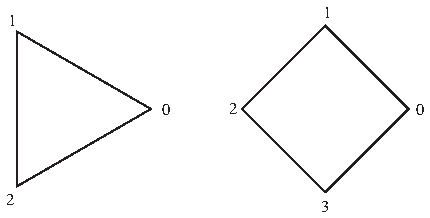
\includegraphics[width=0.590\linewidth,height=.8\textheight,keepaspectratio]{assets/p064_02.pdf}\end{center}
\end{BookFloat}

\noindent We justify calling \BookInline{\langle D_{n},\allowbreak \circ \rangle } a group with Theorem 4.17.

\BookLabel{4.17 Theorem} For any \BookInline{n\geq 3,\allowbreak \langle D_{n},\allowbreak \circ \rangle } is a group.

\BookLabel{\textit{Proof}} We first show that function composition is an operation on \BookInline{D_{n}.} Let \BookInline{\phi,\allowbreak \theta \in D_{n}} and suppose that the line between vertices \BookInline{i} and \BookInline{j} is an edge in \BookInline{P_{n}.} Since \BookInline{\theta \in D_{n},\allowbreak } the line between \BookInline{\theta (i)} and \BookInline{\theta (j)} is an edge of \BookInline{P_{n}.} Because \BookInline{\phi \in D_{n},\allowbreak } and the line between \BookInline{\theta (i)} and \BookInline{\theta (j)} is an edge, the line between \BookInline{\phi (\theta (i))= \phi \circ \theta (i)} and \BookInline{\phi (\theta (j))= \phi \circ \theta (j)} is an edge of \BookInline{P_{n}.}

We leave it to the reader to check that if the line segment between \BookInline{\phi (\theta (i))= \phi \circ \theta (i)} and \BookInline{\phi (\theta (j))= \phi \circ \theta (j)} is an edge of \BookInline{P_{n},\allowbreak } then the line segment between \BookInline{i} and \BookInline{j} is an edge of \BookInline{P_{n}.}

We also know that the composition of one-to-one and onto functions is one-to-one and onto, so \BookInline{\phi \circ \theta \in D_{n}.} Therefore, function composition is an operation on \BookInline{D_{n}.}

The operation of composition of functions is associative, so \BookInline{\mathcal{G}_{1}} is satisfied. The function \BookInline{\iota:\mathbb{Z}_{n}\to \mathbb{Z}_{n}} defined by \BookInline{\iota (k)= k} is an identity in \BookInline{D_{n},\allowbreak } so \BookInline{\mathcal{G}_{2}} is satisfied. Finally, if \BookInline{\phi \in D_{n},\allowbreak } then \BookInline{\phi ^{- 1}\in D_{n};} the inverse function for \BookInline{f} acts as the inverse in the group sense, so \BookInline{\mathcal{G}_{3}} is satisfied. Therefore\BookInline{,\allowbreak \langle D_{n},\allowbreak \circ \rangle } is a group\BookInline{.}\BookEnd{\blacklozenge}

\noindent Following tradition, we will use multiplicative notation in the dihedral groups instead of using \BookInline{\circ.} If the operation on \BookInline{D_{n}} were abelian, we could use additive notation, but in Example 4.18 we find that \BookInline{D_{n}} is not abelian.

\BookLabel{4.18 Example} Let \BookInline{n\geq 3} and \BookInline{\rho:Z_{n}\to Z_{n}} be given by rotating the \BookInline{n-}gon \BookInline{P_{n}} by \BookInline{\frac{2\pi }{n}}, which just rotates each vertex to the next one. That is,

\begin{BookFloat}{04_nonabelian_examples-p64-10}
\begin{center}\small \textbf{4.19 Figure}\end{center}
\begin{center}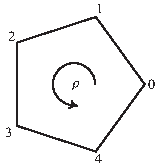
\includegraphics[width=0.220\linewidth,height=.8\textheight,keepaspectratio]{assets/review_v3_p064_4.19.pdf}\end{center}
\end{BookFloat}

\begin{center}\begin{adjustbox}{max width=\linewidth}\BookInline{\displaystyle \rho (k)= k+ _{n}1}\end{adjustbox}\end{center}

\noindent for each \BookInline{k\in \mathbb{Z}_{n},\allowbreak } as can be visualized in Figure 4.19. The function \BookInline{\rho } matches edges to edges and it is one-to-one and onto. So \BookInline{\rho \in D_{n}.}

A second element in \BookInline{D_{n}} is reflection about the \BookInline{x-}axis, which we call \BookInline{\mu.} By glancing at Figure 4.20 we see that in \BookInline{D_{5},\allowbreak \mu (0)= 0,\allowbreak \mu (1)= 4,\allowbreak \mu (2)= 3,\allowbreak \mu (3)= 2,\allowbreak } and \BookInline{\mu (4)= 1.} For any \BookInline{n\geq 3} in general, if \BookInline{k\in \mathbb{Z}_{n},\allowbreak } then

\begin{center}\begin{adjustbox}{max width=\linewidth}\BookInline{\displaystyle \mu (k)= - k.}\end{adjustbox}\end{center}

\noindent (Recall that in \BookInline{\mathbb{Z}_{n},\allowbreak - k} is the additive inverse of \BookInline{k,\allowbreak } which is \BookInline{n- k} for \BookInline{k>0} and \BookInline{- 0= 0.)}

\end{BookBody}

% Source PDF page 65; original printed page 48
\BookSource{65}{48}
\BookNarrativetrue

\begin{BookBody}

Let us check if \BookInline{\mu \rho = \rho \mu.} We start by checking what each function does to 0.

\begin{BookFloat}{04_nonabelian_examples-p65-1}
\begin{center}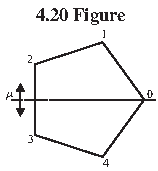
\includegraphics[width=0.217\linewidth,height=.8\textheight,keepaspectratio]{assets/p065_00.pdf}\end{center}
\end{BookFloat}

\begin{center}\begin{adjustbox}{max width=\linewidth}\BookInline{\displaystyle \begin{aligned}\mu (\rho (0))&= \mu (1) \\ &= n- 1\end{aligned}}\end{adjustbox}\end{center}

\begin{center}\begin{adjustbox}{max width=\linewidth}\BookInline{\displaystyle \begin{aligned}\rho (\mu (0))&= \rho (0) \\ &= 1\end{aligned}}\end{adjustbox}\end{center}

\noindent Since \BookInline{n\geq 3,\allowbreak n- 1\neq 1,\allowbreak } which implies that \BookInline{\mu \rho \neq \rho \mu.} Thus for all \BookInline{n\geq 3,\allowbreak D_{n}} is not abelian\BookInline{.}\BookEnd{\blacktriangle}

\BookLabel{4.21 Theorem} Let \BookInline{n\geq 3.} The order of the dihedral group \BookInline{D_{n}} is \BookInline{2n} and

\begin{center}\begin{adjustbox}{max width=\linewidth}\BookInline{\displaystyle D_{n}= \{\iota ,\allowbreak \rho ,\allowbreak \rho ^{2},\allowbreak \rho ^{3},\allowbreak \cdots ,\allowbreak \rho ^{n- 1},\allowbreak \mu ,\allowbreak \mu \rho ,\allowbreak \mu \rho ^{2},\allowbreak \mu \rho ^{3},\allowbreak \cdots ,\allowbreak \mu \rho ^{n- 1}\}.}\end{adjustbox}\end{center}

\BookLabel{\textit{Proof}} We first show there can be at most \BookInline{2n} elements of \BookInline{D_{n}.} If we map the vertices \BookInline{\mathbb{Z}_{n}} to the vertices \BookInline{\mathbb{Z}_{n},\allowbreak } vertex 0 has \BookInline{n} possible images. Let \BookInline{y} be the image of vertex 0. Since \BookInline{y} is connected by an edge to just two vertices, 1 must map to one of these two vertices. So after the image of vertex 0 is determined, there are only two choices for the image of 1. After the images of vertices 0 and 1 are determined, the rest are fixed. This means that there are at most \BookInline{2n} elements of \BookInline{D_{n}.}

To show that \BookInline{|D_{n}|= 2n} we only need to show that no two of the functions \BookInline{\iota = } \BookInline{\rho ^{0},\allowbreak \rho,\allowbreak \rho ^{2},\allowbreak \rho ^{3},\allowbreak...,\allowbreak \rho ^{n- 1},\allowbreak \mu,\allowbreak \mu \rho,\allowbreak \mu \rho ^{2},\allowbreak \mu \rho ^{3},\allowbreak...,\allowbreak \mu \rho ^{n- 1}} are the same. We first suppose that \BookInline{\rho ^{k}= \rho ^{r}} for some integers \BookInline{0\leq k\leq n- 1} and \BookInline{0\leq r\leq n- 1.} Then:

\begin{center}\begin{adjustbox}{max width=\linewidth}\BookInline{\displaystyle \begin{aligned}\rho ^{k}(0)&= \rho ^{r}(0) \\ k+ _{n}0&= r+ _{n}0 \\ k&= r\end{aligned}}\end{adjustbox}\end{center}

\noindent This shows that no two of \BookInline{\iota = \rho ^{0},\allowbreak \rho,\allowbreak \rho ^{2},\allowbreak \rho ^{3},\allowbreak...,\allowbreak \rho ^{n- 1}} are the same.

We next show that no two of \BookInline{\mu = \mu \rho ^{0},\allowbreak \mu \rho,\allowbreak \mu \rho ^{2},\allowbreak \mu \rho ^{3},\allowbreak...,\allowbreak \mu \rho ^{n- 1}} are the same. As before we assume that \BookInline{\mu \rho ^{k}= \mu \rho ^{r}} where \BookInline{0\leq k\leq n- 1} and \BookInline{0\leq r\leq n- 1} are integers. By cancellation, we have \BookInline{\rho ^{k}= \rho ^{r}.} But then \BookInline{k= r} as shown above. Therefore no two of \BookInline{\mu = \mu \rho ^{0},\allowbreak \mu \rho,\allowbreak \mu \rho ^{2},\allowbreak \mu \rho ^{3},\allowbreak...,\allowbreak \mu \rho ^{n- 1}} are the same.

It now only remains to show that there are no values for \BookInline{k} and \BookInline{r} with \BookInline{\rho ^{k}= \mu \rho ^{r}.} Note that traversing the \BookInline{n-}gon in the order

\begin{center}\begin{adjustbox}{max width=\linewidth}\BookInline{\displaystyle \rho ^{k}(0),\allowbreak \rho ^{k}(1),\allowbreak \rho ^{k}(2),\allowbreak \cdots ,\allowbreak \rho ^{k}(n- 1)}\end{adjustbox}\end{center}

\noindent progresses in a counterclockwise manner regardless of which \BookInline{k} we use. On the other hand,

\begin{center}\begin{adjustbox}{max width=\linewidth}\BookInline{\displaystyle \mu \rho ^{k}(0),\allowbreak \mu \rho ^{k}(1),\allowbreak \mu \rho ^{k}(3),\allowbreak \cdots ,\allowbreak \mu \rho ^{k}(n)}\end{adjustbox}\end{center}

\noindent traverses the \BookInline{n-}gon in a clockwise manner. This shows that there are no values of \BookInline{k} and \BookInline{r} for which \BookInline{\rho ^{k}= \mu \rho ^{r}.} Therefore\BookInline{,\allowbreak D_{n}} has at least \BookInline{2n} elements. Combining this with the fact that \BookInline{D_{n}} has at most \BookInline{2n} elements shows that \BookInline{|D_{n}|= 2n} and

\begin{center}\begin{adjustbox}{max width=\linewidth}\BookInline{\displaystyle D_{n}= \{\iota ,\allowbreak \rho ,\allowbreak \rho ^{2},\allowbreak \rho ^{3},\allowbreak \cdots ,\allowbreak \rho ^{n- 1},\allowbreak \mu ,\allowbreak \mu \rho ,\allowbreak \mu \rho ^{2},\allowbreak \mu \rho ^{3},\allowbreak \cdots ,\allowbreak \mu \rho ^{n- 1}\}.}\end{adjustbox}\end{center} \BookEnd{\blacklozenge}

\noindent Theorem 4.21 says that if \BookInline{\phi \in D_{n},\allowbreak } then there is an integer \BookInline{0\leq k\leq n- 1} such that either \BookInline{\phi = \rho ^{k}} or else \BookInline{\phi = \mu \rho ^{k}.} We refer to this representation of \BookInline{\phi } as the\textbf{ standard form}. We notice that each application of \BookInline{\mu } reverses the direction traversed by the images of \BookInline{0,\allowbreak 1,\allowbreak 2,\allowbreak 3,\allowbreak...,\allowbreak n.} We use this fact in the following example.

\BookLabel{4.22 Example} Let \BookInline{n\geq 3.} We know \BookInline{\rho \mu \neq \mu \rho } from Example 4.18, so let us determine \BookInline{\rho \mu \in D_{n}} in standard form. Each time we apply \BookInline{\mu } we reverse the clock direction of the images of \BookInline{0,\allowbreak 1,\allowbreak 2,\allowbreak 3,\allowbreak...,\allowbreak n- 1.} This means that \BookInline{\mu \rho \mu } reverses direction twice, so the rotation is 
% Source PDF page 66; original printed page 49
\BookSource{66}{49}
back to counterclockwise. Thus \BookInline{\mu \rho \mu = \rho ^{k}} for some \BookInline{k.} We determine the value of \BookInline{k} by determining where 0 is sent:

\end{BookBody}

\BookNarrativetrue

\begin{BookBody}

\begin{center}\begin{adjustbox}{max width=\linewidth}\BookInline{\displaystyle k= \rho ^{k}(0)= \mu \rho \mu (0)= \mu \rho (0)= \mu (1)= n- 1}\end{adjustbox}\end{center}

Therefore,

\begin{center}\begin{adjustbox}{max width=\linewidth}\BookInline{\displaystyle \mu \rho \mu = \rho ^{n- 1}.}\end{adjustbox}\end{center}

\noindent Multiplying both sides on the left by \BookInline{\mu } yields:

\begin{center}\begin{adjustbox}{max width=\linewidth}\BookInline{\displaystyle \mu \mu \rho \mu = \mu \rho ^{n- 1}}\end{adjustbox}\end{center}

\noindent Since \BookInline{\mu \mu = \iota,\allowbreak } we conclude that

\begin{center}\begin{adjustbox}{max width=\linewidth}\BookInline{\displaystyle \rho \mu = \mu \rho ^{n- 1}.}\end{adjustbox}\end{center} \BookEnd{\blacktriangle}

\noindent When computing products in \BookInline{D_{n}} we normally want our answer in standard form. This is not difficult if we keep in mind a few basic facts about the group \BookInline{D_{n}.} We have shown some of the properties listed below, and the rest you will be asked to verify in the exercises.

\noindent \BookInline{1.\rho ^{n}= \iota (}Rotation by \BookInline{2\pi } is the identity map.)

\noindent \BookInline{2.(\rho ^{k})^{- 1}= \rho ^{n- k}}

\noindent \BookInline{3.\mu ^{2}= \iota,\allowbreak } which implies \BookInline{\mu ^{- 1}= \mu (}Reflect across a line twice is the identity map.) \BookInline{4.\rho ^{k}\mu = \mu \rho ^{n- k}(}Example 4.22 for \BookInline{k= 1} and Exercise 30 for any \BookInline{k.)}

\BookLabel{4.23 Example} In the group \BookInline{D_{5}} compute \BookInline{(\mu \rho ^{2})(\mu \rho ).} We see that

\begin{center}\begin{adjustbox}{max width=\linewidth}\BookInline{\displaystyle \begin{aligned}(\mu \rho ^{2})(\mu \rho )&= \mu \rho ^{2}\mu \rho  \\ &= \mu (\rho ^{2}\mu )\rho  \\ &= \mu (\mu \rho ^{5- 2})\rho  \\ &= \mu ^{2}\rho ^{4} \\ &= \rho ^{4}\end{aligned}}\end{adjustbox}\end{center} \BookEnd{\blacktriangle}

\BookLabel{4.24 Example} In the dihedral group \BookInline{D_{n}} compute \BookInline{(\mu \rho ^{k})^{- 1}.}

\begin{center}\begin{adjustbox}{max width=\linewidth}\BookInline{\displaystyle \begin{aligned}(\mu \rho ^{k})^{- 1}&= (\rho ^{k})^{- 1}\mu ^{- 1} \\ &= \rho ^{n- k}\mu  \\ &= \mu \rho ^{n- (n- k)} \\ &= \mu \rho ^{k}\end{aligned}}\end{adjustbox}\end{center} \BookEnd{\blacktriangle}

\noindent In Example 4.24 we determined that the inverse of \BookInline{\mu \rho ^{k}} is itself, which suggests that \BookInline{\mu \rho ^{k}} could be reflection across a line of symmetry. In Exercise 37, you will be asked to show this is the case. Geometrically, we can see that each of the elements of the form \BookInline{\mu \rho ^{k}} is reflection across a line. Placing one mirror along the line of reflection for \BookInline{\mu } and another mirror along the line of reflection for \BookInline{\mu \rho } is the basis for designing a kaleidoscope. Any element in \BookInline{D_{n}} can be written as a product using only the elements \BookInline{\mu } and \BookInline{\mu \rho } since we can write \BookInline{\rho = \mu \mu \rho.} In a kaleidoscope successive reflections across the mirrors correspond to taking products involving \BookInline{\mu } and \BookInline{\mu \rho.} So the image you see in the kaleidoscope has all the symmetries in \BookInline{D_{n}.} That is, you can rotate the image by \BookInline{\frac{360^{\circ }}{n}} or reflect it across any one of the lines of reflection for the elements \BookInline{\mu \rho ^{k}.} Figure 4.25 is a typical image from a kaleidoscope with dihedral group \BookInline{D_{16}} symmetries.

\end{BookBody}

% Source PDF page 67; original printed page 50
\BookSource{67}{50}
\BookNarrativefalse

\begin{BookBody}

\begin{BookFloat}{04_nonabelian_examples-p67-0}
\begin{center}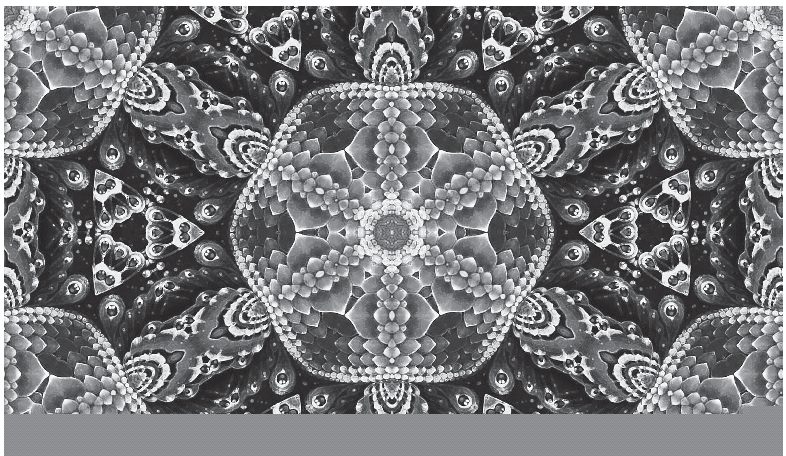
\includegraphics[width=1.000\linewidth,height=.8\textheight,keepaspectratio]{assets/p067_00.pdf}\end{center}
\begin{center}\small\textbf{4.25 Figure}\end{center}
\end{BookFloat}

k c o t s r e t t u h S / n o i t a e r c \_ I Z I

\BookExerciseTitle{4} \BookEnd{\blacksquare}

\BookTextHeading{\textbf{Computation}}

\noindent In Exercises 1 through 5, compute the indicated product involving the following permutations in \BookInline{S_{6}:} \BookInline{\sigma = \begin{pmatrix}1 & 2 & 3 & 4 & 5 & 6 \\3 & 1 & 4 & 5 & 6 & 2\end{pmatrix}}, \BookInline{\tau = \begin{pmatrix}1 & 2 & 3 & 4 & 5 & 6 \\2 & 4 & 1 & 3 & 6 & 5\end{pmatrix}}, \BookInline{\mu = \begin{pmatrix}1 & 2 & 3 & 4 & 5 & 6 \\5 & 2 & 4 & 3 & 1 & 6\end{pmatrix}}.

\BookExercise{1.}{\BookInline{\tau \sigma }}

\BookExercise{2.}{\BookInline{\tau ^{2}\sigma }}

\BookExercise{3.}{\BookInline{\mu \sigma ^{2}}}

\BookExercise{4.}{\BookInline{\sigma ^{- 2}\tau }}

\BookExercise{5.}{\BookInline{\sigma ^{- 1}\tau \sigma }}

\noindent In Exercises 6 through 9, compute the expressions shown for the permutations \BookInline{\sigma,\allowbreak \tau,\allowbreak } and \BookInline{\mu } defined prior to Exercise 1.

\BookExercise{6.}{\BookInline{\sigma ^{6}}}

\BookExercise{7.}{\BookInline{\mu ^{2}}}

\BookExercise{8.}{100 \BookInline{\sigma }}

\BookExercise{9.}{100 \BookInline{\mu }}

\BookExercise{10.}{Convert the permutations \BookInline{\sigma,\allowbreak \tau,\allowbreak } and \BookInline{\mu } defined prior to Exercise 1 to disjoint cycle notation.}

\BookExercise{11.}{Convert the following permutations in \BookInline{S_{8}} from disjoint cycle notation to two-row notation. \textbf{a.} (1, 4, 5)(2, 3) \textbf{b.} (1, 8, 5)(2, 6, 7, 3, 4) \textbf{c.} (1, 2, 3)(4, 5)(6, 7, 8)}

\BookExercise{12.}{Compute the permutation products. \textbf{a.} (1, 5, 2, 4)(1, 5, 2, 3) \textbf{b}\BookInline{.(1,\allowbreak 5,\allowbreak 3)(1,\allowbreak 2,\allowbreak 3,\allowbreak 4,\allowbreak 5,\allowbreak 6)(1,\allowbreak 5,\allowbreak 3)^{- 1}} \textbf{c}\BookInline{.[(1,\allowbreak 6,\allowbreak 7,\allowbreak 2)^{2}(4,\allowbreak 5,\allowbreak 2,\allowbreak 6)^{- 1}(1,\allowbreak 7,\allowbreak 3)]^{- 1}} \textbf{d.} (1, 6)(1, 5)(1, 4)(1, 3)(1, 2)}

\BookExercise{13.}{Compute the following elements of \BookInline{D_{12}.} Write your answer in standard form. \textbf{a}\BookInline{.\mu \rho ^{2}\mu \rho ^{8}} \textbf{b}\BookInline{.\mu \rho ^{10}\mu \rho ^{- 1}} \textbf{c}\BookInline{.\rho \mu \rho ^{- 1}} \textbf{d}\BookInline{.(\mu \rho ^{3}\mu ^{- 1}\rho ^{- 1})^{- 1}}}

\end{BookBody}

% Source PDF page 68; original printed page 51
\BookSource{68}{51}
\BookNarrativefalse

\begin{BookBody}

\BookExercise{14.}{Write the group table for \BookInline{D_{3}.} Compare the group tables for \BookInline{D_{3}} and \BookInline{S_{3}.} Are the groups isomorphic?}

Let \BookInline{A} be a set and let \BookInline{\sigma \in S_{A}.} For a fixed \BookInline{a\in A,\allowbreak } the set

\begin{center}\begin{adjustbox}{max width=\linewidth}\BookInline{\displaystyle \mathcal{O}_{a,\allowbreak \sigma }= \{\sigma ^{n}(a)\mid n\in \mathbb{Z}\}}\end{adjustbox}\end{center}

is the\textbf{ orbit} of \BookInline{a} \textbf{under} \BookInline{\sigma.} In Exercises 15 through 17, find the orbit of 1 under the permutation defined prior to Exercise 1.

\BookExercise{15.}{\BookInline{\sigma }}

\BookExercise{16.}{\BookInline{\tau }}

\BookExercise{17.}{\BookInline{\mu }}

\BookExercise{18.}{Verify that \BookInline{H= \{\iota,\allowbreak \mu,\allowbreak \rho ^{2},\allowbreak \mu \rho ^{2}\}\subseteq D_{4}} is a group using the operation function composition.}

\BookExercise{19.}{\textbf{. a} Verify that the six matrices}

\begin{center}\begin{adjustbox}{max width=\linewidth}\BookInline{\displaystyle \begin{bmatrix} 1 & 0 & 0 \\ 0 & 1 & 0 \\ 0 & 0 & 1 \end{bmatrix},\allowbreak  \begin{bmatrix} 0 & 1 & 0 \\ 0 & 0 & 1 \\ 1 & 0 & 0 \end{bmatrix},\allowbreak  \begin{bmatrix} 0 & 0 & 1 \\ 1 & 0 & 0 \\ 0 & 1 & 0 \end{bmatrix},\allowbreak  \begin{bmatrix} 1 & 0 & 0 \\ 0 & 0 & 1 \\ 0 & 1 & 0 \end{bmatrix},\allowbreak  \begin{bmatrix} 0 & 0 & 1 \\ 0 & 1 & 0 \\ 1 & 0 & 0 \end{bmatrix},\allowbreak  \begin{bmatrix} 0 & 1 & 0 \\ 1 & 0 & 0 \\ 0 & 0 & 1 \end{bmatrix}}\end{adjustbox}\end{center}

form a group under matrix multiplication. [\textit{Hint}: Don’t try to compute all products of these matrices. Instead, think how the column vector \BookInline{\begin{bmatrix} 0 \\ 1 \\ 2 \end{bmatrix}} is transformed by multiplying it on the left by each of the matrices.]

\BookExercise{b.}{What group discussed in this section is isomorphic to this group of six matrices?}

\BookExercise{20.}{After working Exercise 18, write down eight matrices that form a group under matrix multiplication that is isomorphic to \BookInline{D_{4}.}}

\BookTextHeading{\textbf{Concepts}}

\noindent In Exercises 21 through 23, correct the definition of the italicized term without reference to the text, if correction is needed, so that it is in a form acceptable for publication.

\BookExercise{21.}{The\textit{ dihedral group} \BookInline{D_{n}} is the set of all functions \BookInline{\phi:\mathbb{Z}_{n}\to \mathbb{Z}_{n}} such that the line segment between vertex \BookInline{i} and vertex \BookInline{j} of \BookInline{U_{n}} is an edge of \BookInline{P_{n}} if and only if the line segment between vertices \BookInline{\phi (i)} and \BookInline{\phi (j)} in \BookInline{U_{n}} is an edge of \BookInline{P_{n}.}}

\BookExercise{22.}{A\textit{ permutation} of a set \BookInline{S} is a one-to-one map from \BookInline{S} to \BookInline{S.}}

\BookExercise{23.}{The\textit{ order} of a group is the number of elements in the group.}

\noindent In Exercises 24 through 28, determine whether the given function is a permutation of \BookInline{\mathbb{R}.}

\BookExercise{24.}{\BookInline{f_{1}:\mathbb{R}\to \mathbb{R}} defined by \BookInline{f_{1}(x)= x+ 1}}

\BookExercise{25.}{\BookInline{f_{2}:\mathbb{R}\to \mathbb{R}} defined by \BookInline{f_{2}(x)= x^{2}}}

\BookExercise{26.}{\BookInline{f_{3}:\mathbb{R}\to \mathbb{R}} defined by \BookInline{f_{3}(x)= - x^{3}}}

\BookExercise{27.}{\BookInline{f_{4}:\mathbb{R}\to \mathbb{R}} defined by \BookInline{f_{4}(x)= e^{x}}}

\BookExercise{28.}{\BookInline{f_{5}:\mathbb{R}\to \mathbb{R}} defined by \BookInline{f_{5}(x)= x^{3}- x^{2}- 2x}}

\BookExercise{29.}{Determine whether each of the following is true or false.}

\BookExercise{a.}{Every permutation is a one-to-one function.}

\BookExercise{b.}{Every function is a permutation if and only if it is one-to-one.}

\BookExercise{c.}{Every function from a finite set onto itself must be one-to-one.}

\BookExercise{d.}{Every subset of an abelian group \BookInline{G} that is also a group using the same operation as \BookInline{G} is abelian.}

\BookExercise{e.}{The symmetric group \BookInline{S_{10}} has 10 elements.}

\BookExercise{f.}{If \BookInline{\phi \in D_{n},\allowbreak } then \BookInline{\phi } is a permutation on the set \BookInline{\mathbb{Z}_{n}.}}

\BookExercise{g.}{The group \BookInline{D_{n}} has exactly \BookInline{n} elements.}

\BookExercise{h.}{\textbf{h}\BookInline{.D_{3}} is a subset of \BookInline{D_{4}.}}

\BookTextHeading{\textbf{Theory}}

\BookExercise{30.}{Let \BookInline{n\geq 3} and \BookInline{k\in \mathbb{Z}_{n}.} Prove that in \BookInline{D_{n},\allowbreak \rho ^{k}\mu = \mu \rho ^{n- k}.}}

\BookExercise{31.}{Show that \BookInline{S} is a nonabelian group for \BookInline{n\geq 3.}}

\end{BookBody}

% Continuation on source PDF page 69, preceding Section 5
\BookNarrativefalse

\begin{BookBody}

\BookExercise{32.}{Strengthening Exercise 31, show that if \BookInline{n\geq 3,\allowbreak } then the only element of \BookInline{\sigma } of \BookInline{S_{n}} satisfying \BookInline{\sigma \gamma = \gamma \sigma } for all \BookInline{\gamma \in S_{n}} is \BookInline{\sigma = \iota,\allowbreak } the identity permutation.}

\BookExercise{33.}{Orbits were defined before Exercise 15. Let \BookInline{a,\allowbreak b\in A} and \BookInline{\sigma \in S_{A}.} Show that if \BookInline{\mathcal{O}_{a,\allowbreak \sigma }} and \BookInline{\mathcal{O}_{b,\allowbreak \sigma }} have an element in common, then \BookInline{\mathcal{O}_{a,\allowbreak \sigma }= \mathcal{O}_{b,\allowbreak \sigma }.}}

\BookExercise{34.}{(See the warning following Theorem 4.8.) Let \BookInline{G} be a group with binary operation \BookInline{\ast.} Let \BookInline{G^{\prime }} be the same set as \BookInline{G,\allowbreak } and define a binary operation \BookInline{\ast ^{\prime }} on \BookInline{G^{\prime }} by \BookInline{x\ast ^{\prime }y= y\ast x} for all \BookInline{x,\allowbreak y\in G^{\prime }.}}

\BookExercise{a.}{(Intuitive argument that \BookInline{G^{\prime }} under \BookInline{\ast ^{\prime }} is a group.) Suppose the front wall of your classroom were made of transparent glass, and that all possible products \BookInline{a\ast b= c} and all possible instances \BookInline{a\ast (b\ast c)= } \BookInline{(a\ast b)\ast c} of the associative property for \BookInline{G} under \BookInline{\ast } were written on the wall with a magic marker. What would a person see when looking at the other side of the wall from the next room in front of yours?}

\BookExercise{b.}{Show from the mathematical definition of \BookInline{\ast ^{\prime }} that \BookInline{G^{\prime }} is a group under \BookInline{\ast ^{\prime }.}}

\BookExercise{35.}{Give a careful proof using the definition of isomorphism that if \BookInline{G} and \BookInline{G^{\prime }} are both groups with \BookInline{G} abelian and \BookInline{G^{\prime }} not abelian, then \BookInline{G} and \BookInline{G^{\prime }} are not isomorphic.}

\BookExercise{36.}{Prove that for any integer \BookInline{n\geq 2,\allowbreak } there are at least two nonisomorphic groups with exactly \BookInline{2n} elements.}

\BookExercise{37.}{Let \BookInline{n\geq 3} and \BookInline{0\leq k\leq n- 1.} Prove that the map \BookInline{\mu \rho ^{k}\in D_{n}} is reflection about the line through the origin that makes an angle of \BookInline{- \frac{\pi k}{n}} with the \BookInline{x- }axis.}

\BookExercise{38.}{Let \BookInline{n\geq 3} and \BookInline{k,\allowbreak r\in \mathbb{Z}_{n}.} Based on Exercise 37, determine the element of \BookInline{D_{n}} that corresponds to first reflecting across the line through the origin at an angle of \BookInline{- \frac{2\pi k}{n}} and then reflection across the line through the origin making an angle of \BookInline{- \frac{2\pi r}{n}.} Prove your answer.}

\end{BookBody}
\ifdefined\BookMaster\let\BookFinish\relax\else\def\BookFinish{\end{document}}\fi\BookFinish
